\section{三维 A–φ 场与诊断}
\label{chapter:08}

% block-id: 08.aphi.p1
\hypertarget{08.aphi.p1}{}
A–φ 模型按 \eqref{eq:E07}，由保存的 A 和 φ 的实际梯度恢复电流。圆柱三档网格分别含 1683、3672、9108 节点，结果见 图~\ref{fig:aphi_gates}。最细档径向 J 校准达到目标，φ 与规范残差在三档中仍未通过，较粗两档 J 也未达到目标。制造解检查支持所检验方程与实现的对应关系，物理圆柱校准则揭示了仍需研究的场势一致性问题。

% block-id: 08.aphi.p2
\hypertarget{08.aphi.p2}{}
图~\ref{fig:aphi_preserved} 使用 128 个具有明确身份的节点样本，分别显示 A、φ、J 和实际 φ 梯度，表示这些采样位置的数值。边界、缩放、导数与后处理的诊断记录，以及直接分解、OOC 和迭代路线的失败原因，共同保留在复现资料中。它们用于进一步区分实现问题与离散误差；当前圆柱结果的物理验收状态为未通过。

% block-id: 08.equation.E07
\hypertarget{08.equation.E07}{}
\hypertarget{E07}{}\begin{equation}\mathbf J=-\sigma\left(j\omega\mathbf A+\nabla\phi\right)\tag{8}\label{eq:E07}\end{equation}

% block-id: 08.figure.aphi_preserved
\hypertarget{08.figure.aphi_preserved}{}
\begin{figure}[!htbp]
\centering
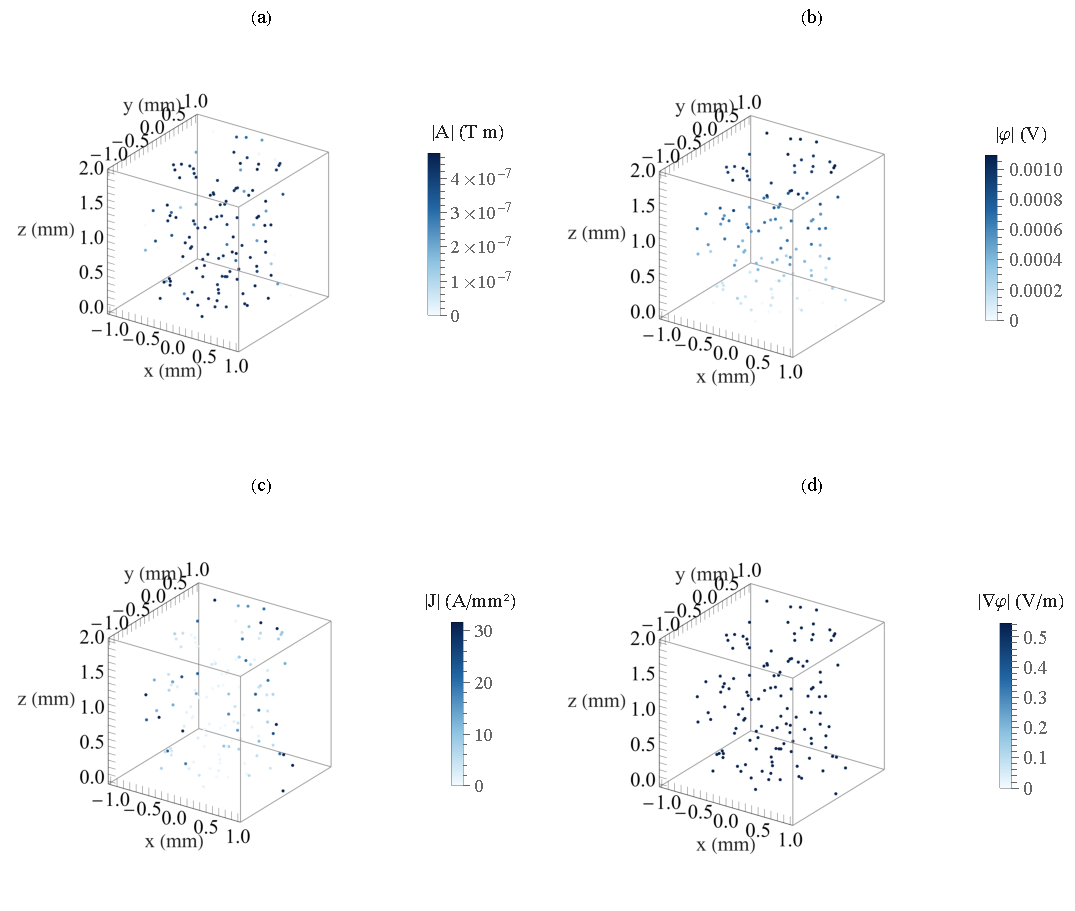
\includegraphics[width=\linewidth,height=.72\textheight,keepaspectratio]{../../assets/zh-CN/aphi_preserved.pdf}
\caption{A–φ 保存场样本。 面板分别给出 A、φ、J 和实际 φ 梯度。 128 个指定节点保留其样本身份。色标使用实际保存的复数场与导数幅值。}
\label{fig:aphi_preserved}
\end{figure}

% block-id: 08.figure.aphi_gates
\hypertarget{08.figure.aphi_gates}{}
\begin{figure}[!htbp]
\centering
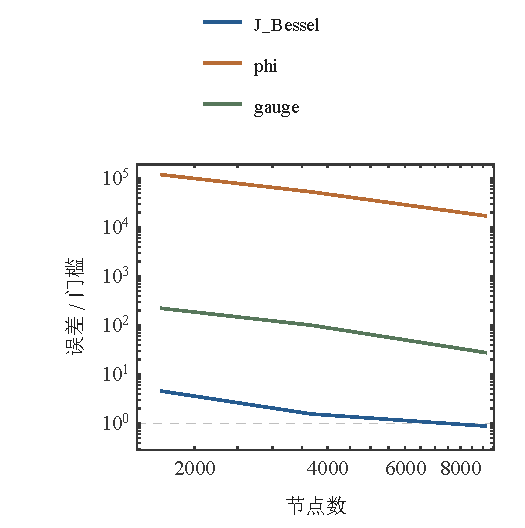
\includegraphics[width=\linewidth,height=.72\textheight,keepaspectratio]{../../assets/zh-CN/aphi_gates.pdf}
\caption{A–φ 圆柱校准指标。 三档网格与各指标门槛分别展示。 圆柱三档含 1683、3672、9108 节点。误差以各自验收门槛归一化，水平线标出单位比值。}
\label{fig:aphi_gates}
\end{figure}
